\documentclass[tikz,border=4pt]{standalone}
\usepackage{amsmath}
\begin{document}
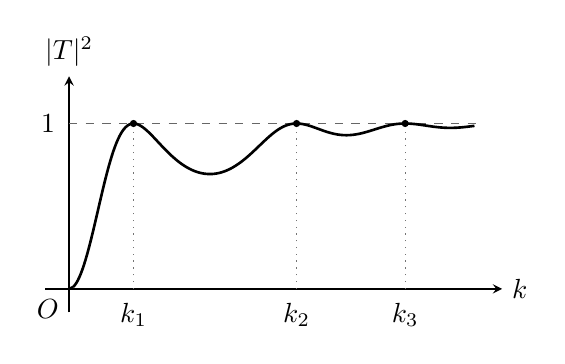
\begin{tikzpicture}[>=stealth, thick, scale=1.0]
  % Axes
  \draw[->, line width=0.5pt] (-0.3, 0) -- (5.5, 0) node[right] {$k$};
  \draw[->, line width=0.5pt] (0, -0.3) -- (0, 2.7) node[above] {$|T|^2$};
  \node[below left] at (0, 0) {$O$};

  % Horizontal asymptote |T|^2 = 1 at y = 2.1
  \draw[dashed, line width=0.5pt, black!60] (0, 2.1) -- (5.2, 2.1);
  \node[left] at (-0.05, 2.1) {$1$};

  % Let k a = 3 x, k0 a = 9.1 => c = (k0 a / 3)^2 = 9.20111, c^2 / 4 = 21.1651
  % Resonances:
  % p a = 3 pi => k1 a = 2.4526 => x1 = 0.8175
  % p a = 4 pi => k2 a = 8.6662 => x2 = 2.8887
  % p a = 5 pi => k3 a = 12.8035 => x3 = 4.2678
  \draw[line width=0.95pt, domain=0.05:5.15, samples=260]
    plot (\x, {2.1 / (1 + (21.1651 / (\x*\x)) / (\x*\x + 9.2011) * (sin(deg(3*sqrt(\x*\x + 9.2011))))^2)});
  \draw[line width=0.95pt] (0, 0) -- (0.05, {2.1 / (1 + (21.1651 / 0.0025) / (0.0025 + 9.2011) * (sin(deg(3*sqrt(0.0025 + 9.2011))))^2)});

  % Resonance tick marks k1, k2, k3
  \foreach \xr/\lbl in {0.818/$k_1$, 2.889/$k_2$, 4.268/$k_3$} {
    \draw[dotted, line width=0.45pt, black!55] (\xr, 0) -- (\xr, 2.1);
    \fill (\xr, 2.1) circle (1.3pt);
    \node[below] at (\xr, -0.05) {\lbl};
  }
\end{tikzpicture}
\end{document}
